% \documentclass{article}

% % Language setting
% % Replace `english' with e.g. `spanish' to change the document language
% \usepackage[english, russian]{babel}

% % Set page size and margins
% % Replace `letterpaper' with `a4paper' for UK/EU standard size
% \usepackage[letterpaper,top=2cm,bottom=2cm,left=3cm,right=3cm,marginparwidth=1.75cm]{geometry}

% % Useful packages
% \usepackage{amsmath}
% \usepackage{color}
% \usepackage{xcolor}
% \usepackage[dvipsnames]{xcolor}
% \usepackage{graphicx}
% \usepackage[colorlinks=true, allcolors=blue]{hyperref}
% \usepackage{color}   %May be necessary if you want to color links
% \usepackage{hyperref}
% \hypersetup{
%     colorlinks=true, %set true if you want colored links
%     linktoc=all,     %set to all if you want both sections and subsections linked
%     linkcolor=blue,  %choose some color if you want links to stand out
% }
\documentclass{article}

% Language setting
% Replace `english' with e.g. `spanish' to change the document language
\usepackage[english]{babel}
\usepackage{amsmath}

%графика
\usepackage{wrapfig}
\usepackage{graphicx}
\usepackage{pgfplots}
\usepackage{tikz}


\usepackage{tcolorbox}

% Set page size and margins
% Replace `letterpaper' with `a4paper' for UK/EU standard size
\usepackage[letterpaper,top=2cm,bottom=2cm,left=3cm,right=3cm,marginparwidth=1.75cm]{geometry}

% Useful packages
\usepackage{amsmath}
\usepackage{amssymb}
\usepackage{graphicx}
\usepackage{fixltx2e}
\usepackage[colorlinks=true, allcolors=blue]{hyperref}

\usepackage{geometry}
\geometry{left=25mm,right=25mm,
 top=25mm,bottom=25mm}

\title{Exotic Options}
\author{Bidva Maxim}
% Колонтитулы
\usepackage{fancyhdr}
\pagestyle{fancy}
\renewcommand{\headrulewidth}{0.1mm}  
\renewcommand{\footrulewidth}{0.1mm}
\lfoot{}
\rfoot{\thepage}
\cfoot{}
\rhead{CMF-2022}
\chead{}




\begin{document}
\maketitle
\tableofcontents
\newpage
\section{EXOTIC DERIVATIVES}

{\bf Exotic derivatives} are traded only OTC and used (in contrast to vanilla):

\begin{multicols}
    \begin{itemize}
        \item to fit specific firm need for hedging
        \item to address tax or regulatory concerns
        \item for speculation(on interest rate, exchange rates, commodities prices)
    \end{itemize}
\end{multicols}
\
Main issues:
\begin{multicols}
    \begin{itemize}
        \item Complex payoffs should be thoroughly understood by customers
        \item Hedging tends to be difficult
        \item Reliable pricing model
        \item Position closure
    \end{itemize}
\end{multicols}
\section{ZERO-COST PRODUCTS}
\begin{itemize}

    \item A {\bf package} - combination of standard European options, forwards, cash and the underlying asset.\\ 
    Examples: bull/bear spreads, straddles, strangles etc.\\
    \item Any derivative can be constructed into a {\bf zero-cost} product to be paid in arrears.\

    \begin{itemize}
        \item Let's take a derivative with maturity T and premium f. Instead of paying premium upfront - it can be structured to be paid at maturity with compounding $f(1 + R)^T$
        \item Example of European call option -> after conversion to zero-cost payoff is: $\max(S_T - K - A, - A)$, where A = $c(1 + R)^T$ and c is normal call premium
    \end{itemize}

\end{itemize}
\section{NONSTANDARD AMERICAN OPTIONS}
{\bf Nonstandard American Options:}
\begin{itemize}
    \item OTC market 
    \item Exchange-traded

\end{itemize}
Various flavors:

\begin{itemize}
    \item Bermudan option - can be exercised only on specific dates
    \item Restricted exercise period feature (lockout period) Example employee stock options.
    \item Variable strike (e.g. strike depends on time) Example callable bond
\end{itemize}\\
Revaluation - Binomial trees can be used to value American options
\newpage
\section{GAP OPTIONS}


Has 2 strikes - $K_1$ and $K_2$
\begin{itemize}
    \item {\bf Gap call option} (European) $I_{S_T > K_2} (S_T - K_1)$
    \begin{itemize}
        \item $K_2 > K_1$: nonnegative
        \item $K_2 < K_1$: can be negative
    \end{itemize}
\end{itemize}\\
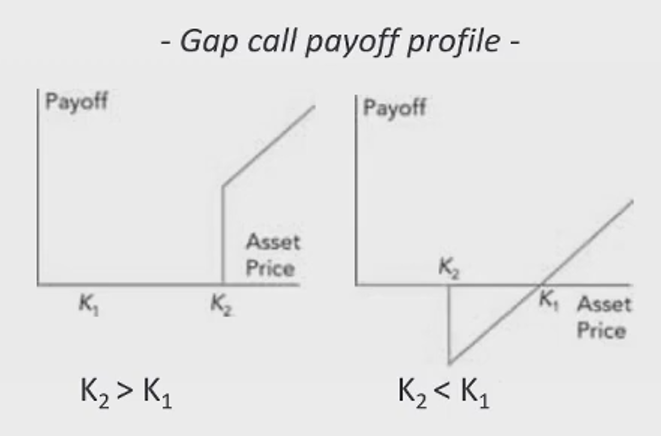
\includegraphics[width=0.55\textwidth]{Gap_call_payoff_profile.png}\\


\begin{itemize}
    \item {\bf Gap put option} (European) $I_{S_T < K_2} ( K_1 - S_T)$
    \begin{itemize}
        \item $K_2 < K_1$: nonnegative
        \item $K_2 > K_1$: can be negative
    \end{itemize}
\end{itemize}


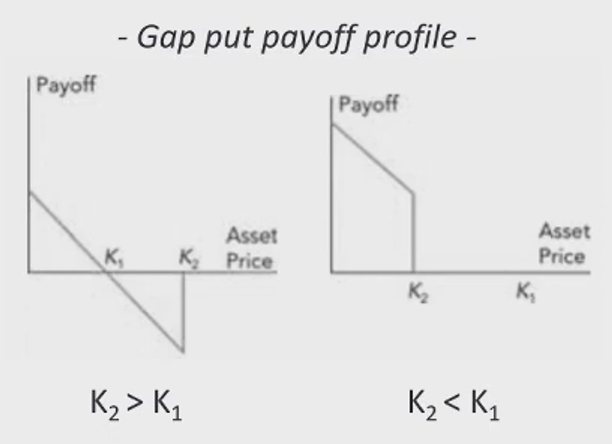
\includegraphics[width=0.55\textwidth]{Gap_put_payoff_profile.png}



\newpage
\section{FORWARD START OPTION}
\begin{itemize}
    \item Option comes into existence on a prespecified date in the future
    \item Strike in {\bf not fixed in advance} usually ATM when starting
    \item Example: employee stock options if employer promises that they will be granted on future dates
    \item {\bf Valuation} Mathematical formula for forward start option starting at time $T_1$ and maturing at time $T_2$:
    \begin{itemize}
        \item Its value at time $T_1$ is $c \frac{S_1}{S_0}$
        \item Its value today at $T_0$ is $c e^{-q T_1}$ where $q$ is dividend yield $c$ is the value of ATM option with a life of ($T_2 - T_1$)
        \item For non-div paying stock $q = 0$ ATM forward start option price equals vanilla option price with the same life
    \end{itemize}
\end{itemize}
\section{CLIQUET ANS CHOOSER OPTIONS}
{\bf Cliquet option} is a series of forward start options with certain rules to determine strike prices. It could consist of 3 options:
\begin{multicols}
    \begin{itemize}
        \item 1 year vanilla option
        \item 1 year forward start option (starting in 1 year)
        \item 1 year forward start option (starting in 2 year)
    \end{itemize}
\end{multicols}
{\bf Chooser option} allows the holder to choose whether the option is a call or a put after a certain period of time ($T_1$)
\begin{multicols}
    \begin{itemize}
        \item Can be considered as package of call and put options with different strikes and time to maturity
        \item Value of choose option then $max(c, p)$ where $c$ is price of call, $p$ - put
        \item Rewriting $max(c, p) = c + max(0, p - c) = c + max(0, PV(K) - S_1)$ and $PV$ denotes present value from $T_2$ to $T_1$
        \item It means that chooser option is a package consisting of:
        \begin{itemize}
         \item Call option with strike K and maturing at $T_2$
         \item Put option with strike PV(K) maturing at $T_1$
       \end{itemize}
    \end{itemize}
\end{multicols}
\section{COMPOUND OPTIONS}
{\bf Compound option} - option on another option.\\
\begin{center}
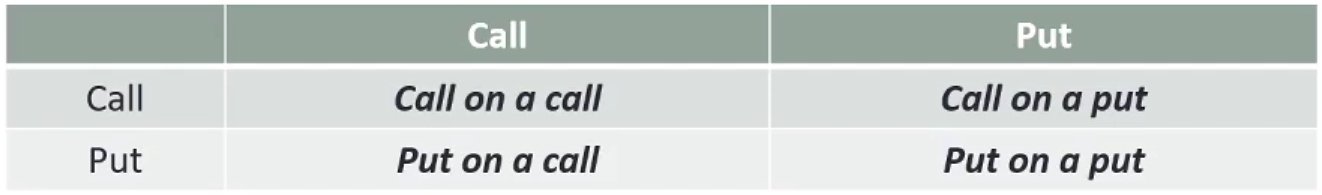
\includegraphics[width=0.85\textwidth]{Compound_option.png}\\
\end{center}
{\bf Example of a call on  a call:}\\
The holder has a right to pay $K_1$ at time $T_1$ to purchase a long position in a call on an underlying. The latter allows to buy an asset for $K_2$ at time $T_2$
{\bf Features:}
\begin{itemize}
        \item The value of an underlying option is determined by the value of the underlying asset
        \item More leverage compared to vanilla options
        \item More sensitive to volatility than ordinary options
    \end{itemize}
\section{BARRIER OPTIONS}
{\bf Barrier options} have payoff dependent on whether the underlying asset reaches certain barrier level.\\
\begin{center}
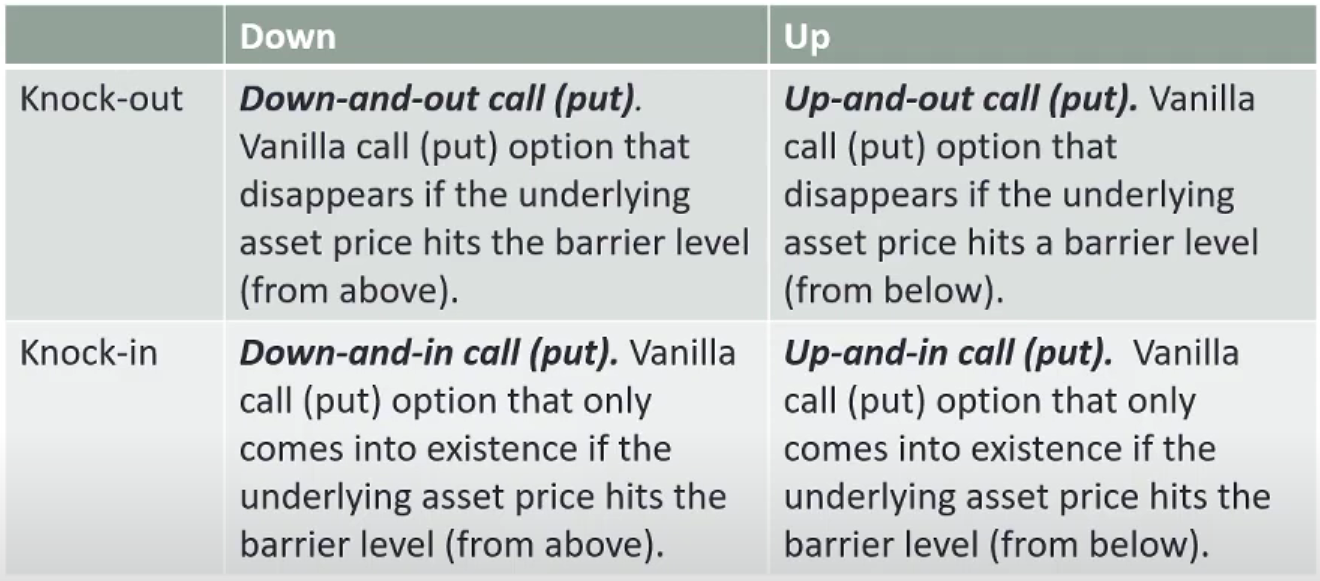
\includegraphics[width=0.85\textwidth]{Barrier_options.png}
\end{center}
{\bf Parisian options} asset price must remain above/below the barrier for a specified number of days\\
{\bf Barrier options} features:
\begin{itemize}
    \item Path-dependent  - depends on whether a barrier is reached 
    \item less expensive than standard options -which is attractive for buyers
    \item No-arbitrage equalities have to be respected for barrier options:\\
    $c = c_{do} + c_{di}, c = c_{uo} + c_{ui}, p = p_{do} + p_{di}, p = p_{uo} + p_{ui}$
    \item Example:When barrier level is equal to strike $\rightarrow$ $c = c_{ui}$
    \item Frequency of barrier observation increases $\rightarrow$ what is impact on KI and KO option values? \\KI increases, KO decreases
    \item For down-and-out and up-and-out options Vega becomes negative. This is contrary to ordinary option vega behaviour? When spot price is close to barrier level the probability that barrier will be hit increases $\rightarrow$ value decreases
\end{itemize}
\newpage
\section{BINARY OPTIONS}
{\bf Binary options} - options with discontinuous payoff profiles \\(discontinuity of payoff creates an incentive for underlying price manipulation close to expiry)
\begin{itemize}
    \item {\bf Cash-or-nothing call/put} pays the value of the stock when the contract is initiated if the stock price
    \item {\bf Asset-or-nothing call/put} pays the value of the stock when the contract is initiated if the stock price ends up in-the-money at expiration.
    \item European call/put options can be decomposed in a package of binary cash-or-nothing and asset-or nothing options
\end{itemize}
\begin{figure}[h]
\centering
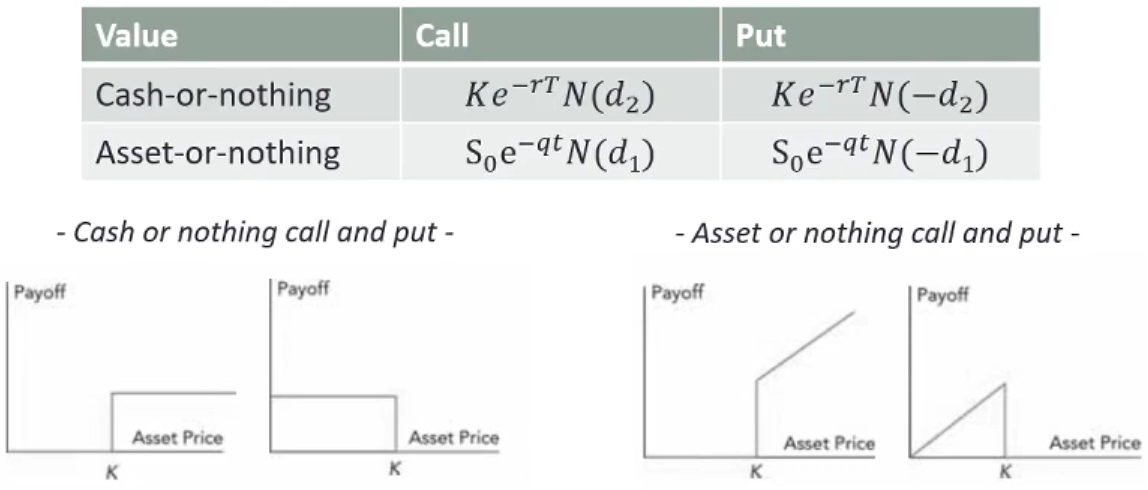
\includegraphics[width=0.85\textwidth]{Binary_opritons.png}\\
\end{figure}

\section{LOOKBACK OPTIONS}
{\bf Lookback options} are options hose payoffs depend on the maximum or minimum price of the underlying asset during the life of the option\\
\begin{center}
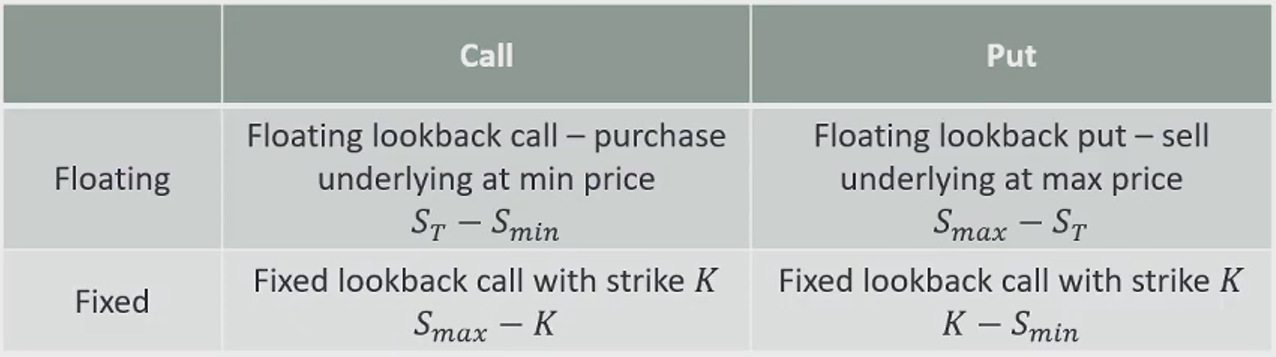
\includegraphics[width=0.75\textwidth]{Lookback_options.png}
\end{center}
where $S_{min}/S_{max}$ - min/max price during life of option, $S_T$ -is underlying price at expiry
\begin{itemize}
    \item Lookback options are more expensive than ordinary ones
    \item The value of a lookback option depends on how often the spot prices is observed 
    \item What is the impact of spot price observation increase on the value of lookback option?
    \item Fixed lookback call or put is like an American option where investor pretends to choose the best possible exercise date
\end{itemize}
\section{ASIAN OPTIONS}
{\bf Average price} call and put options pay the difference between the average stock price and the strike price.
\begin{itemize}
    \item Average price call payoff $\max(0, S_A - K)$
    \item Average price put payoff $\max(0, K - S_A)$
\end{itemize}
Where $S_A$ stands for spot average\\
{\bf Average strike} options pay the difference between the average stock price and the final asset price (average represents a strike).
\begin{itemize}
    \item Average price call payoff $\max(0, S_T - S_A)$
    \item Average price put payoff $\max(0, S_A - S_T)$
\end{itemize}
Where $S_T$ is spot price at maturity T and $S_A$ stands for spot average during the life of option\\
{\bf Features:} 
\begin{itemize}
    \item Asian options are less expensive then regular ones with similar maturity/strike 
    \item Average strike options guarantee that the average price paid for an asset is not greater than the final price (or average price received is not less)
\end{itemize}
\section{MULTIPLE ASSET OPTIONS}
\begin{itemize}
    \item {\bf Exchange option} - option to exchange one asset for another.
    \begin{itemize}
    \item Example to buy euros for dollars from point of view of Russian investor is an exchange option.
    \end{itemize}
    \item Consider a European option to give up an asset worth $U_T$ at time T for an asset worth $V_T$.\\
    The payoff is $\max(V_T - U_T, 0)$
    \item This option can be prices in BSM framework
    \item Position in exchange option can be then valued as per below\\
    $\max(U_T, V_T) = U_T + \max(V_T - U_T, 0)$
    \item {\bf Basket option} - underlying is a basket of asset. Assets can be stocks, currencies, stock indices etc.
    \item Potentially a good hedging instrument for those seeking to reduce costs by hedging their aggregate exposure to several assets
    \Rainbow option are options involving 2 or more risky assets
\end{itemize}

\section{VOLATILITY/VARIANCE SWAPS}
\begin{itemize}
    \item {\bf Volatility swap} - exchange of fixed pre-specified volatility ($\sigma_K$) vs realized vol ($\sigma$) multiplied by some notional ($L_vol$): $L_{vol}(\sigma - \sigma_K)$
    \item Volatility swap is used when a trader needs to take a position dependent only on volatility.
    \bigskip
    \item {\bf Variance swap} - exchange of fixed variance $V_K$ vs realized variance $\sigma^2$ multiplied by some national $L_{var}: L_{var}(\sigma^2 - V_K)$
    \item Variance swaps are easier to value than volatility swaps because they can be replicated using calls and puts.
\end{itemize}
\section{HEDGING EXOTICS}
\begin{itemize}
    \item Some exotic options are easier to hedge (e.g. Asian options)
    \item Other options such as barrier - more difficult, esp near barrier
    \item 2 types of hedging:
    \begin{itemize}
        \item {\bf Dynamic options replication} - replicating portfolio is adjusted continuously\\ (e.g. Greeks hedging)
    \end{itemize}
    \item {\bf Static options replication} principle - 2 portfolios having the same value on boundary (S and T) must also be worth the same at all interior points $\rightarrow$ the goal is to find a portfolio of vanillas matching the exotic value on boundary
    \item Static option replication hedge can be left unchanged until the boundary reached. The trader must unwind the hedge portfolio and create a new hedge.
\end{itemize}

\section{KEY TAKEAWAYS}
\begin{itemize}
    \item Many various types of exotic options design
    \item We have discussed several most basic ones but many more exist
    \item Valuation of exotic options can be a very advanced topic. \\For some of the analytic formula exists, for others - numerical techniques
    \item Exotic options can be good hedge (Asian, basket options etc)
    \item They can be used to speculate on the particular view of the market\\ (compound option, barrier options etc)
    \item Generally exotic options are less competitively priced than vanillas
    \item Specific part of exotic options market take vol/variance swaps
    \item Exotic options can be difficult to hedge hence a specific procedure static option replication was developed for this task which is alternative to Greek letter hedging
    \item Main idea of static replication is find a portfolio of vanillas whose value matches the value of exotic on a boundary
\end{itemize}


\end{document}
